\documentclass[10pt,a4paper]{article}
\usepackage[T1]{fontenc}
\usepackage[utf8]{inputenc}
\usepackage[scaled=0.92]{helvet}
\renewcommand{\familydefault}{\sfdefault}
\usepackage[a4paper,left=2cm,right=2cm,top=1.9cm,bottom=2.3cm]{geometry}
\usepackage[table]{xcolor}
\usepackage{graphicx,booktabs,array,longtable,enumitem,fancyhdr,titlesec,float}
\usepackage[hyphens]{url}
\Urlmuskip=0mu plus 1mu
\renewcommand{\contentsname}{}
\usepackage[font=small,labelfont=bf,labelsep=period,textfont=bf,justification=raggedright,singlelinecheck=false,skip=4pt]{caption}
\usepackage[colorlinks=true,linkcolor=navy,urlcolor=navy,citecolor=navy]{hyperref}
\urlstyle{same}
\definecolor{navy}{HTML}{1F3A5F}
\definecolor{accent}{HTML}{EB6834}
\definecolor{zebra}{HTML}{F2F5F9}
\definecolor{boxbg}{HTML}{FFF4D6}
\definecolor{greyink}{HTML}{52514E}
\setlength{\tabcolsep}{4pt}
\renewcommand{\arraystretch}{1.25}
\setlength{\parskip}{5pt}\setlength{\parindent}{0pt}
\setlist[itemize]{leftmargin=1.2em,itemsep=2pt,topsep=2pt}
\titleformat{\section}{\color{navy}\bfseries\Large}{\thesection.}{0.6em}{}
\titleformat{\subsection}{\color{navy}\bfseries\large}{\thesubsection}{0.6em}{}
\titlespacing*{\section}{0pt}{14pt}{6pt}
\titlespacing*{\subsection}{0pt}{9pt}{4pt}
\setcounter{secnumdepth}{2}
\setcounter{tocdepth}{1}
\pagestyle{fancy}\fancyhf{}
\renewcommand{\headrulewidth}{0pt}
\renewcommand{\footrulewidth}{0.4pt}
\fancyfoot[L]{\footnotesize\color{greyink}Rajasthan and Sikkim: demographic and health-economic profiles (NSS 80th Round, Health)}
\fancyfoot[R]{\footnotesize\color{greyink}Page \thepage}
\hypersetup{pdftitle={Demographic and Health-Economic Profiles of Rajasthan and Sikkim (NSS 80th Round, 2025)},pdfauthor={Group project report}}
\usepackage{graphicx}
\usepackage[usenames]{color, xcolor} 
\usepackage{booktabs}
% \usepackage{float}
\usepackage{ragged2e}
\graphicspath{{figures/}}
\definecolor{urlblue}{RGB}{0,90,160}
\definecolor{citegreen}{RGB}{0,160,90}
\usepackage[
colorlinks = true,
linkcolor = urlblue, 
urlcolor = red, 
citecolor = citegreen
]{hyperref}
\usepackage{latexsym,epsfig,amsmath,amssymb,amsthm,amsfonts,bbm}
\usepackage{fullpage}
\usepackage{enumerate}
\usepackage{tikz}
%\usepackage{titlesec}
\usepackage{setspace}
\usepackage{mathrsfs}
\usepackage{svg}
\usepackage{caption}
\usepackage{changepage}
\usepackage{lipsum}
% \usepackage{enumitem}
\usepackage[utf8]{inputenc} 
% \usepackage[top = 1.5cm, left = 3cm, right = 3cm]{geometry}
\usepackage{enumerate}
\newcommand{\id}{\operatorname{id}}
\usepackage{comment}

% hint environment
\newenvironment{hint}
  {\color{gray}\itshape\textsc{Hint.}\vspace{0.1cm}}
  {\par}


%section environment


\theoremstyle{plain}
\newtheorem{theorem}{Theorem}[section]

\theoremstyle{definition}
\newtheorem{problem}[theorem]{\textsc{Problem}}
\newtheorem*{solution}{Solution}

%for fonts and stuff
\usepackage{amsfonts, amsmath, amssymb, amsthm}
% \usepackage{lmodern}
\usepackage{newtxtext, mathpazo}
% \usepackage{mathpazo}
% \usepackage{bookman}
% \usepackage{kpfonts, euler}





% Commands for mathbb and mathcal
% Blackboard bold
\newcommand{\bA}{\mathbb{A}}
\newcommand{\bB}{\mathbb{B}}
\newcommand{\bC}{\mathbb{C}}
\newcommand{\bD}{\mathbb{D}}
\newcommand{\bE}{\mathbb{E}}
\newcommand{\bF}{\mathbb{F}}
\newcommand{\bG}{\mathbb{G}}
\newcommand{\bH}{\mathbb{H}}
\newcommand{\bI}{\mathbb{I}}
\newcommand{\bJ}{\mathbb{J}}
\newcommand{\bK}{\mathbb{K}}
\newcommand{\bL}{\mathbb{L}}
\newcommand{\bM}{\mathbb{M}}
\newcommand{\bN}{\mathbb{N}}
\newcommand{\bO}{\mathbb{O}}
\newcommand{\bP}{\mathbb{P}}
\newcommand{\bQ}{\mathbb{Q}}
\newcommand{\bR}{\mathbb{R}}
\newcommand{\bS}{\mathbb{S}}
\newcommand{\bT}{\mathbb{T}}
\newcommand{\bU}{\mathbb{U}}
\newcommand{\bV}{\mathbb{V}}
\newcommand{\bW}{\mathbb{W}}
\newcommand{\bX}{\mathbb{X}}
\newcommand{\bY}{\mathbb{Y}}
\newcommand{\bZ}{\mathbb{Z}}

% Calligraphic
\newcommand{\cA}{\mathcal{A}}
\newcommand{\cB}{\mathcal{B}}
\newcommand{\cC}{\mathcal{C}}
\newcommand{\cD}{\mathcal{D}}
\newcommand{\cE}{\mathcal{E}}
\newcommand{\cF}{\mathcal{F}}
\newcommand{\cG}{\mathcal{G}}
\newcommand{\cH}{\mathcal{H}}
\newcommand{\cI}{\mathcal{I}}
\newcommand{\cJ}{\mathcal{J}}
\newcommand{\cK}{\mathcal{K}}
\newcommand{\cL}{\mathcal{L}}
\newcommand{\cM}{\mathcal{M}}
\newcommand{\cN}{\mathcal{N}}
\newcommand{\cO}{\mathcal{O}}
\newcommand{\cP}{\mathcal{P}}
\newcommand{\cQ}{\mathcal{Q}}
\newcommand{\cR}{\mathcal{R}}
\newcommand{\cS}{\mathcal{S}}
\newcommand{\cT}{\mathcal{T}}
\newcommand{\cU}{\mathcal{U}}
\newcommand{\cV}{\mathcal{V}}
\newcommand{\cW}{\mathcal{W}}
\newcommand{\cX}{\mathcal{X}}
\newcommand{\cY}{\mathcal{Y}}
\newcommand{\cZ}{\mathcal{Z}}

\begin{document}

\begin{titlepage}
    \centering
    \vspace*{0.2cm}


    \includesvg[width=0.17\textwidth]{isi-logo.svg}\par
    \vspace{0.4cm}
    {\Large \textsc{Indian Statistical Institute, Kolkata}}\par
    \vspace{0.1cm}
    {\large \textsc{Bachelor of Statistics}}\par

    \vspace{0.5cm}
    \rule{\textwidth}{0.8pt}\par
    \vspace{0.4cm}


    {\large \itshape Economic Statistics and Demography \textbullet{} Project Report}\par
    \vspace{0.5cm}
    {\LARGE \bfseries \textsc{Storytelling with Data:}}\par
    \vspace{0.25cm}
    {\Large \textsc{A Comparative Demographic and Economic Study of\\ Sikkim and Rajasthan}}\par

    \vspace{0.4cm}
    \rule{\textwidth}{0.8pt}\par
    \vspace{0.6cm}
    {\large
    \begin{tabular}{c c}
        Shounak Kar (BS2439)    & Sayan Kar (BS2436) \\[0.2cm]
        Ahan Chakraborty (BS2402) & Arnab Sanyal (BS2411)
    \end{tabular}\par}

    \vspace{0.5cm}
    {\large \textbf{Advisor:} Prof. Kajori Banerjee}\par
    \vspace{0.2cm}
    {\large 12\textsuperscript{th} October 2026}\par

    \vspace{0.8cm}
    
    \begin{minipage}{0.88\textwidth}
        \centering
        {\large \textbf{Abstract}}\par
        \vspace{1cm}
        \justifying
        \small
        \noindent
        

This study examines demographic change, gender differences in health, household consumption and health-financing coverage in Rajasthan and Sikkim using survey-weighted microdata from the NSS 80th Round Health Survey (2025). The two states differ substantially in age structure, household size, marriage patterns and women's educational attainment. Age-standardised chronic-ailment prevalence is broadly similar across states and between men and women. However, hospitalisation patterns reveal an important gender contrast: in Rajasthan, women aged outside 15–49 have lower hospitalisation rates than men, despite comparable reported morbidity, a finding that warrants further investigation. Median monthly per-capita consumption expenditure is higher in Sikkim, although overall consumption inequality is similar in the two states. The largest contrast concerns reported health-financing coverage, estimated at 77.2\% in Rajasthan and 18.6\% in Sikkim. Coverage in Rajasthan is distributed relatively evenly across consumption groups, whereas Sikkim exhibits a more pronounced, though statistically imprecise, concentration among richer households. These findings illustrate important differences in demographic structure, gender-related outcomes and reported health-scheme coverage, while highlighting the limitations of cross-sectional data for drawing causal conclusions about healthcare access and policy effectiveness.\par
    \end{minipage}

    \vfill
\end{titlepage}
\newpage
\section*{Contents}
\vspace{-6pt}
\tableofcontents
\vspace{6pt}
\newpage
\section{Introduction and choice of states}

The project brief asks each group to select two states or union territories and describe their demographic and economic dynamics with empirical data, using tools such as rates and ratios, fertility scenarios, life tables, inequality measures and policy evaluation. We chose Rajasthan and Sikkim because they contrast on almost every dimension the brief lists: size, age structure, fertility, gender differentials and, most relevant for a policy comparison, the way health care is financed.


Published context suggests a clear policy difference. Rajasthan introduced the Chiranjeevi health insurance scheme in May 2021 as a scheme offering universal health cover to Rajasthani families, with the cover amount later raised from Rs 10 lakh to Rs 25 lakh; reports also describe a plan to merge it with Ayushman Bharat PM-JAY [3]. Sikkim launched AB-PMJAY in 2018 alongside the Mukhya Mantri Jeevan Raksha Kosh, a referral-based financial-assistance scheme for treatment outside the state, renamed in 2022 [4]. These are secondary sources and the scheme details may have changed; the survey itself records only broad categories (for example ``State Health Insurance Scheme''), so we cannot match respondents to named schemes. We therefore treat the policy comparison as descriptive.


\textbf{Questions.} (1) How do the two states differ in age structure, fertility, marriage and schooling? (2) Are there gender gaps in health and in access to care? (3) How do consumption levels and inequality compare? (4) How equitably is health-scheme coverage distributed, and is coverage related to hospital use?


\section{Data and methods}

\subsection{Data}

We use unit-level data from the NSS 80th Round survey on Household Social Consumption: Health, collected from January to December 2025 [1]. For each state we were given a single file in which each row is one household member, combining household variables (Level 1: Blocks 1, 2 and 5, including household size, religion, social group and usual consumer expenditure) with person variables (Level 2: Block 3, including age, sex, marital status, education, hospitalisation, ailments and health-scheme coverage). The accompanying data layout and block-code workbooks were used to decode every variable (Appendix A).


\begin{table}[!htb]\centering
\caption{Sample size}
\rowcolors{2}{white}{zebra}
\begin{tabular}{>{\raggedright\arraybackslash}p{6.72cm}>{\raggedright\arraybackslash}p{4.72cm}>{\raggedright\arraybackslash}p{4.72cm}}
\toprule
\rowcolor{navy}\textcolor{white}{\textbf{}} & \textcolor{white}{\textbf{Rajasthan}} & \textcolor{white}{\textbf{Sikkim}} \\
\midrule
\textbf{Households} & 7,642 & 1,033 \\
\textbf{Persons} & 39,878 & 4,237 \\
\textbf{First-stage units (FSUs)} & 959 & 130 \\
\textbf{Persons: rural / urban} & 22,215 / 17,663 & 2,701 / 1,536 \\
\textbf{Women aged 15--49} & 10,484 & 1,250 \\
\textbf{Children aged 0--4} & 4,445 & 376 \\
\bottomrule
\end{tabular}
\begin{minipage}{\textwidth}\par\vspace{2pt}{\footnotesize\itshape Notes: 33 persons in Rajasthan and 5 in Sikkim are recorded as transgender; they are kept in totals but excluded from male/female comparisons. 43 Rajasthan persons have missing ailment and coverage fields and are dropped from those indicators only.\par}\end{minipage}
\end{table}

\subsection{Weights, design and uncertainty}

Every estimate uses the supplied final weight (the survey multiplier divided by 100), which is constant within a household. Weighting matters here: the survey over-samples households with a recent hospitalisation, so the unweighted hospitalised share in the sample is 14.7\% in Rajasthan and 18.9\% in Sikkim, whereas the weighted rates are 3.9\% and 3.1\%. We do not use the weighted totals (67.8 million persons in Rajasthan, 0.63 million in Sikkim) as population counts, only for shares, rates and ratios.


Standard errors account for the stratified cluster design (FSUs within strata) through a Rao-Wu rescaled bootstrap with 500 replicates [5]; 95\% intervals are the estimate plus or minus 1.96 bootstrap standard errors. Comparisons between states treat the two samples as independent. Adjusted odds ratios come from weighted logistic regressions with standard errors clustered by FSU. We report many comparisons, so isolated borderline results should be read cautiously.


\subsection{Measures}

\begin{table}[!htb]\centering
\caption{Definitions}
\rowcolors{2}{white}{zebra}
\begin{tabular}{>{\raggedright\arraybackslash}p{3.42cm}>{\raggedright\arraybackslash}p{13.02cm}}
\toprule
\rowcolor{navy}\textcolor{white}{\textbf{Measure}} & \textcolor{white}{\textbf{Definition}} \\
\midrule
\textbf{MPCE} & Household usual consumer expenditure in a month (purchases, home-grown and in-kind consumption, plus clothing and durables spread over 12 months) divided by household size. Person-weighted. This comes from a health survey and is not comparable with the household consumption expenditure survey. \\
\textbf{Quintiles} & Person-weighted MPCE quintiles formed within each state (Q1 poorest 20\% of that state). They rank households within a state; they do not equalise living standards across states. \\
\textbf{Dependency ratios} & Persons aged 0--14 (young) and 60+ (old) per person aged 15--59. \\
\textbf{Sex ratio} & Females per 1,000 males. \\
\textbf{SMAM} & Singulate mean age at marriage (Hajnal method) from the proportions never married at ages 15--49 and 50 [6]. \\
\textbf{Fertility index (TFI)} & Five times the sum of age-specific shares of women aged 15--49 who report a pregnancy in the Block 3 item ``whether pregnant''. We read this as a pregnancy in the past year (including a continuing one), by analogy with the Block 4 wording; the layout does not state the reference period. It is a proxy for the total fertility rate, not an exact measure. \\
\textbf{Age-standardised rate} & Direct standardisation over eight age bands (0--4, 5--14, 15--24, ..., 55--64, 65+) using the average of the two states' age distributions as the standard, so differences are not due to age structure. \\
\textbf{Female/male ratio} & Ratio of age-standardised female and male rates (parity = 1). For education we use parity indices (female share divided by male share). \\
\textbf{Gini, Lorenz curve} & Computed on person-weighted MPCE [7]. \\
\textbf{Concentration index} & Twice the covariance between an indicator and fractional MPCE rank, divided by the indicator's mean. Positive: concentrated among richer persons; negative: among poorer. For chronic ailment and hospitalisation it is indirectly standardised for age and sex [7, 8]. \\
\textbf{Health-scheme coverage} & Block 3 item on coverage by any health financing scheme or insurance (one code recorded per person): AB-PMJAY, State Health Insurance Scheme, ESIS, central or state employee schemes, employer insurance, privately purchased insurance only, or not covered. \\
\bottomrule
\end{tabular}
\end{table}

\subsection{Quality assurance}

Headline estimates (sex ratio, median age, coverage shares, Gini, standardised hospitalisation rates, the fertility index, SMAM and the concentration index of coverage) were recomputed with an independent implementation, including an exact pairwise Gini, and agreed to at least six significant digits.

\newpage
\section{Demographic profile}

This section describes who lives in each state: the age and sex structure, household size and composition, and religious and social-group make-up. Table 3 lists the indicators and Figure 1 shows the age-sex pyramids.


\begin{table}[!htb]\centering
\caption{Demographic profile (estimate with 95\% CI)}
\rowcolors{2}{white}{zebra}
\begin{tabular}{>{\raggedright\arraybackslash}p{6.62cm}>{\raggedright\arraybackslash}p{4.77cm}>{\raggedright\arraybackslash}p{4.77cm}}
\toprule
\rowcolor{navy}\textcolor{white}{\textbf{Indicator}} & \textcolor{white}{\textbf{Rajasthan}} & \textcolor{white}{\textbf{Sikkim}} \\
\midrule
Rural share of persons (\%) & 72.7 [70.0, 75.5] & 74.4 [66.4, 82.5] \\
Median age (years) & 27.0 [26.2, 27.8] & 32.0 [30.8, 33.2] \\
Mean age (years) & 30.1 [29.7, 30.6] & 33.0 [32.0, 34.1] \\
Persons aged 0--14 (\%) & 25.3 [24.2, 26.4] & 16.4 [13.9, 18.9] \\
Persons aged 15--59 (\%) & 64.4 [63.3, 65.6] & 76.3 [73.2, 79.3] \\
Persons aged 60+ (\%) & 10.3 [9.5, 11.0] & 7.4 [5.4, 9.3] \\
Young dependency ratio & 0.39 [0.37, 0.42] & 0.21 [0.18, 0.25] \\
Old-age dependency ratio & 0.16 [0.15, 0.17] & 0.10 [0.07, 0.12] \\
Total dependency ratio & 0.55 [0.52, 0.58] & 0.31 [0.26, 0.36] \\
Share of population aged 0--4 (\%) & 6.9 & 2.7 \\
Sex ratio, all ages (females per 1,000 males) & 973 [940, 1005] & 871 [794, 947] \\
Sex ratio, rural & 1004 [963, 1044] & 937 [856, 1019] \\
Sex ratio, urban & 895 [840, 950] & 700 [548, 853] \\
Sex ratio, ages 15--59 & 964 [927, 1001] & 880 [785, 974] \\
Household size (mean) & 4.53 [4.42, 4.64] & 3.38 [3.14, 3.62] \\
Female-headed households (\%) & 13.1 [11.4, 14.8] & 16.0 [11.0, 21.0] \\
Hindu (\%) & 89.5 [87.4, 91.6] & 69.0 [62.1, 76.0] \\
Muslim (\%) & 8.8 [6.8, 10.8] & 2.5 [0.5, 4.5] \\
Buddhist (\%) & 0.0 [0.0, 0.0] & 21.9 [15.5, 28.3] \\
Christian (\%) & 0.0 [0.0, 0.0] & 6.5 [3.3, 9.7] \\
Scheduled Tribe (\%) & 13.5 [11.3, 15.7] & 33.6 [27.0, 40.2] \\
Scheduled Caste (\%) & 18.9 [16.4, 21.3] & 6.7 [3.3, 10.1] \\
Other Backward Class (\%) & 50.4 [47.4, 53.4] & 51.1 [43.5, 58.7] \\
Others (\%) & 17.2 [15.1, 19.3] & 8.5 [4.6, 12.5] \\
\bottomrule
\end{tabular}
\begin{minipage}{\textwidth}\par\vspace{2pt}{\footnotesize\itshape Notes: dependency ratios are per person aged 15--59. Religion and social-group shares are of persons, by household characteristics; Sikh and Jain shares in Rajasthan are about 1\% each.\par}\end{minipage}
\end{table}
\begin{figure}[h]
    \centering
    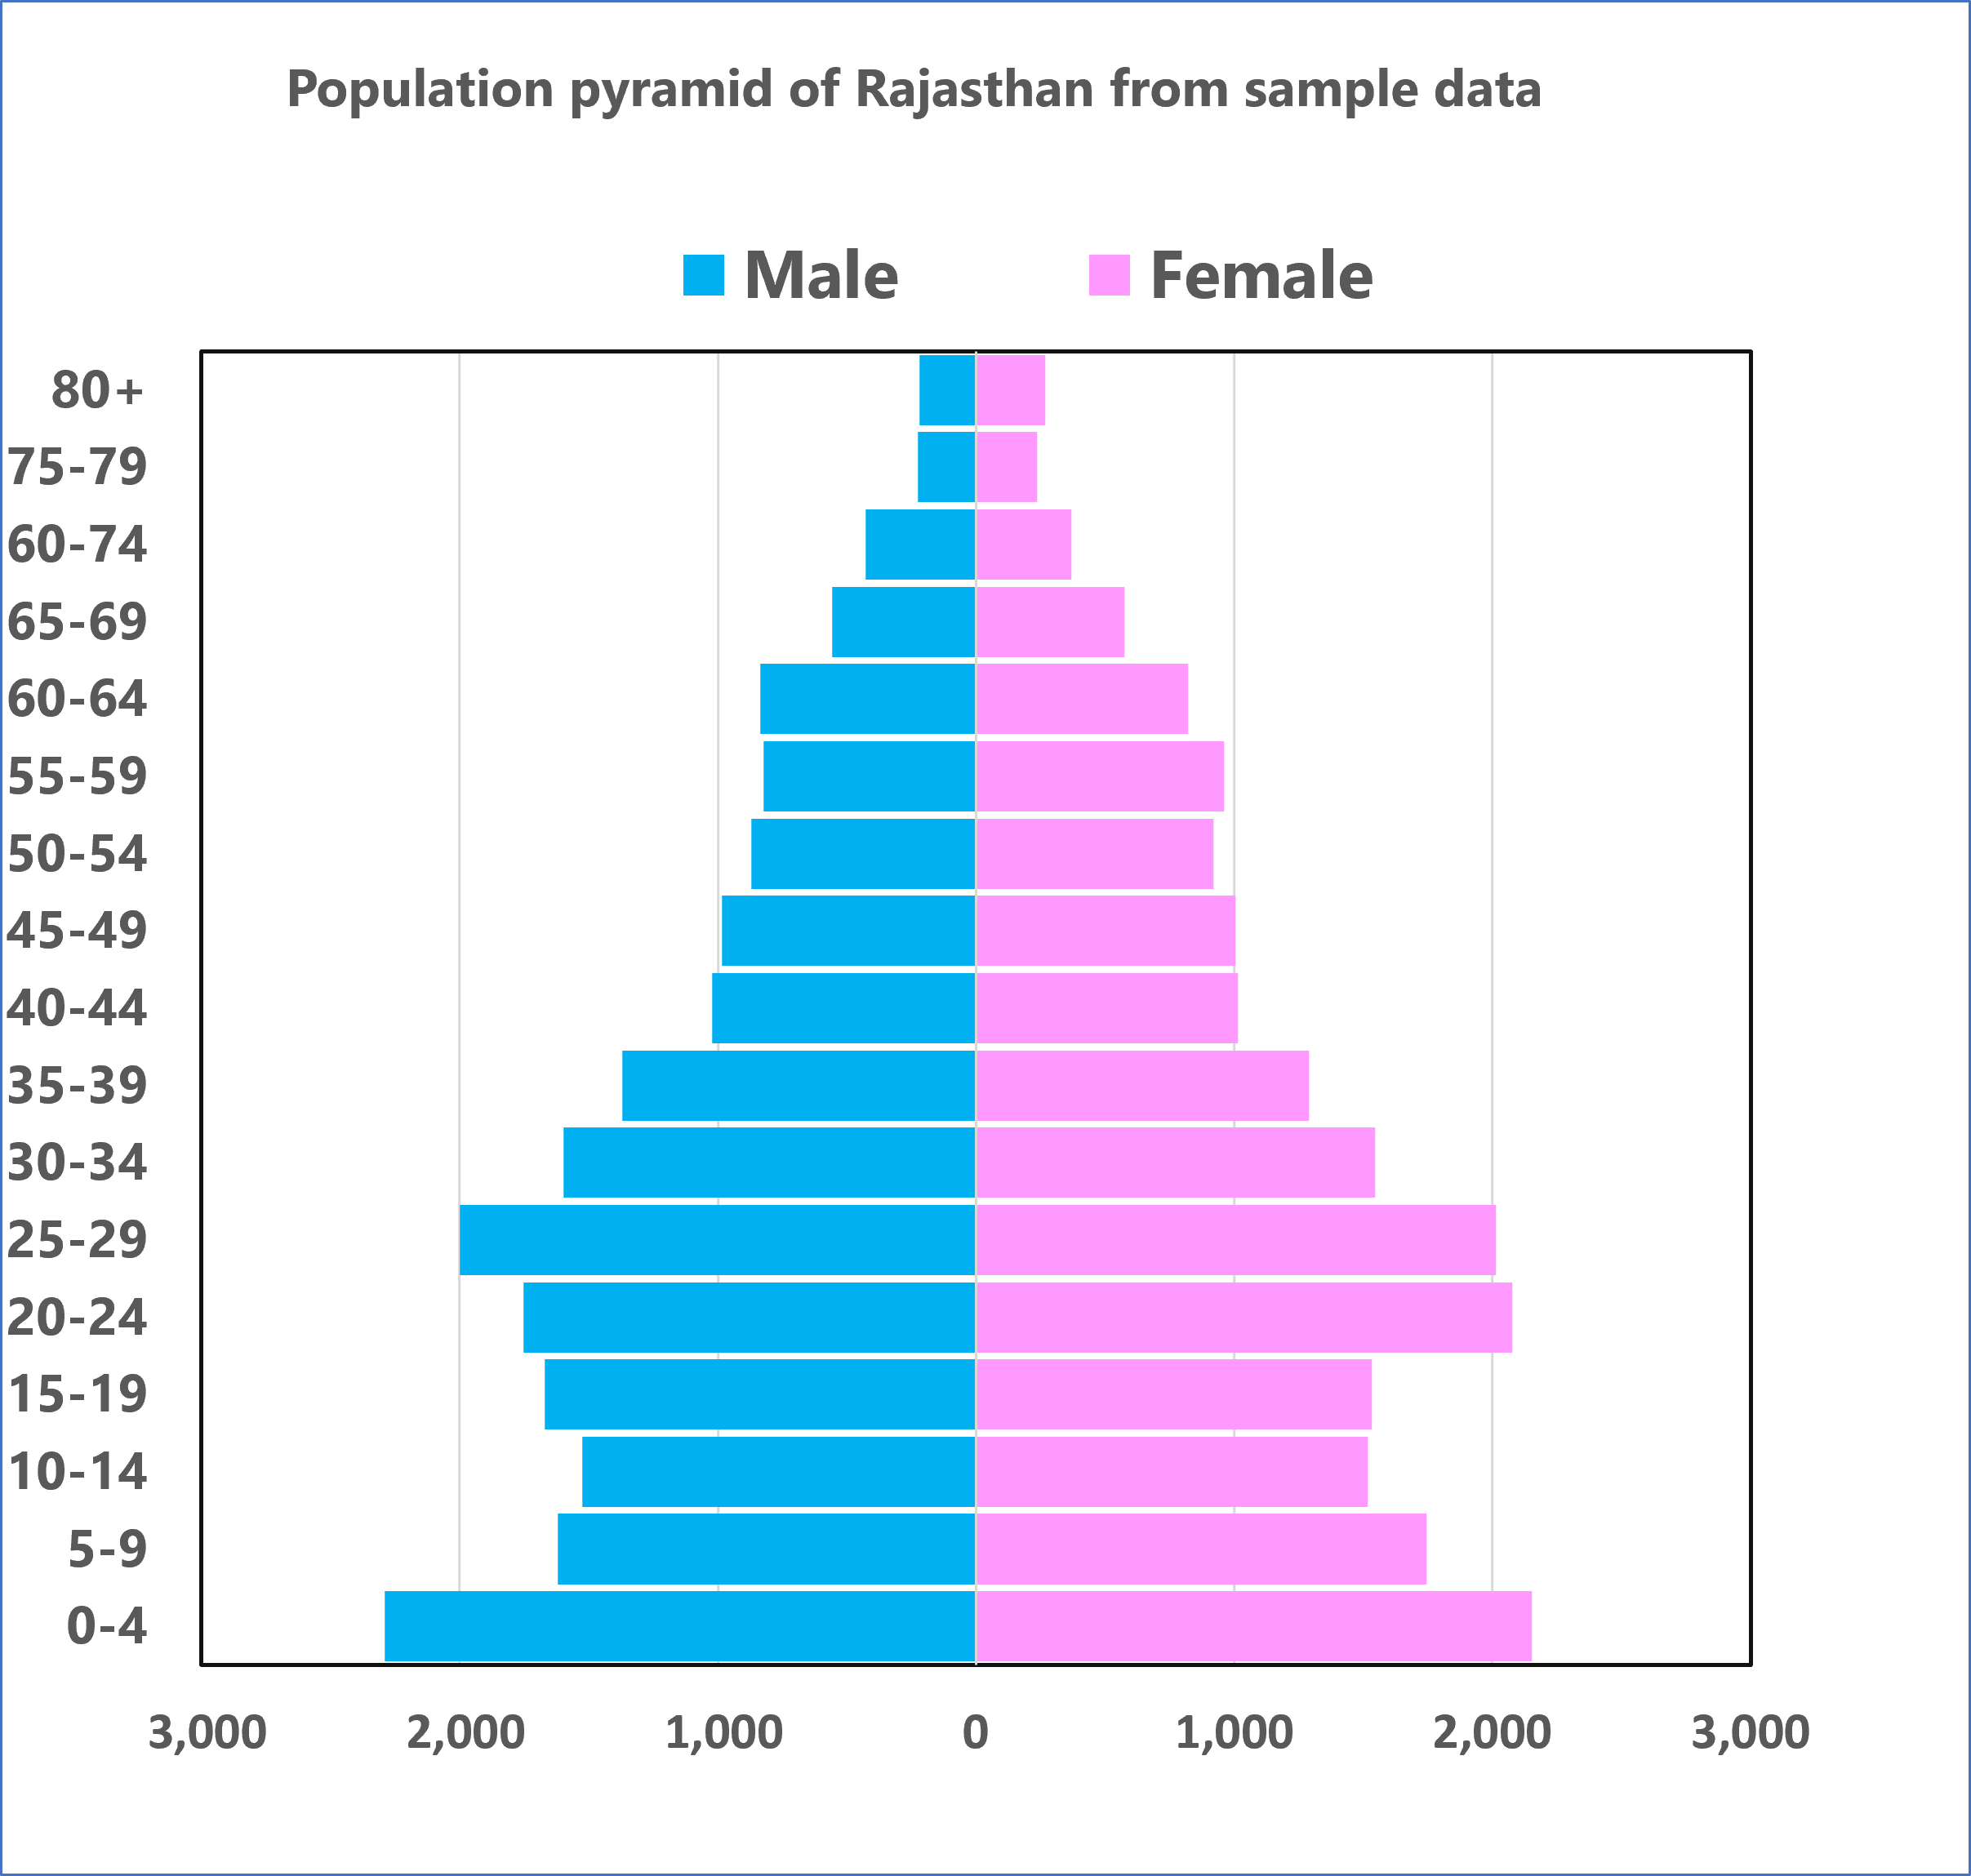
\includegraphics[width=0.46\linewidth]{rajpyramid.png}
    \hfill
    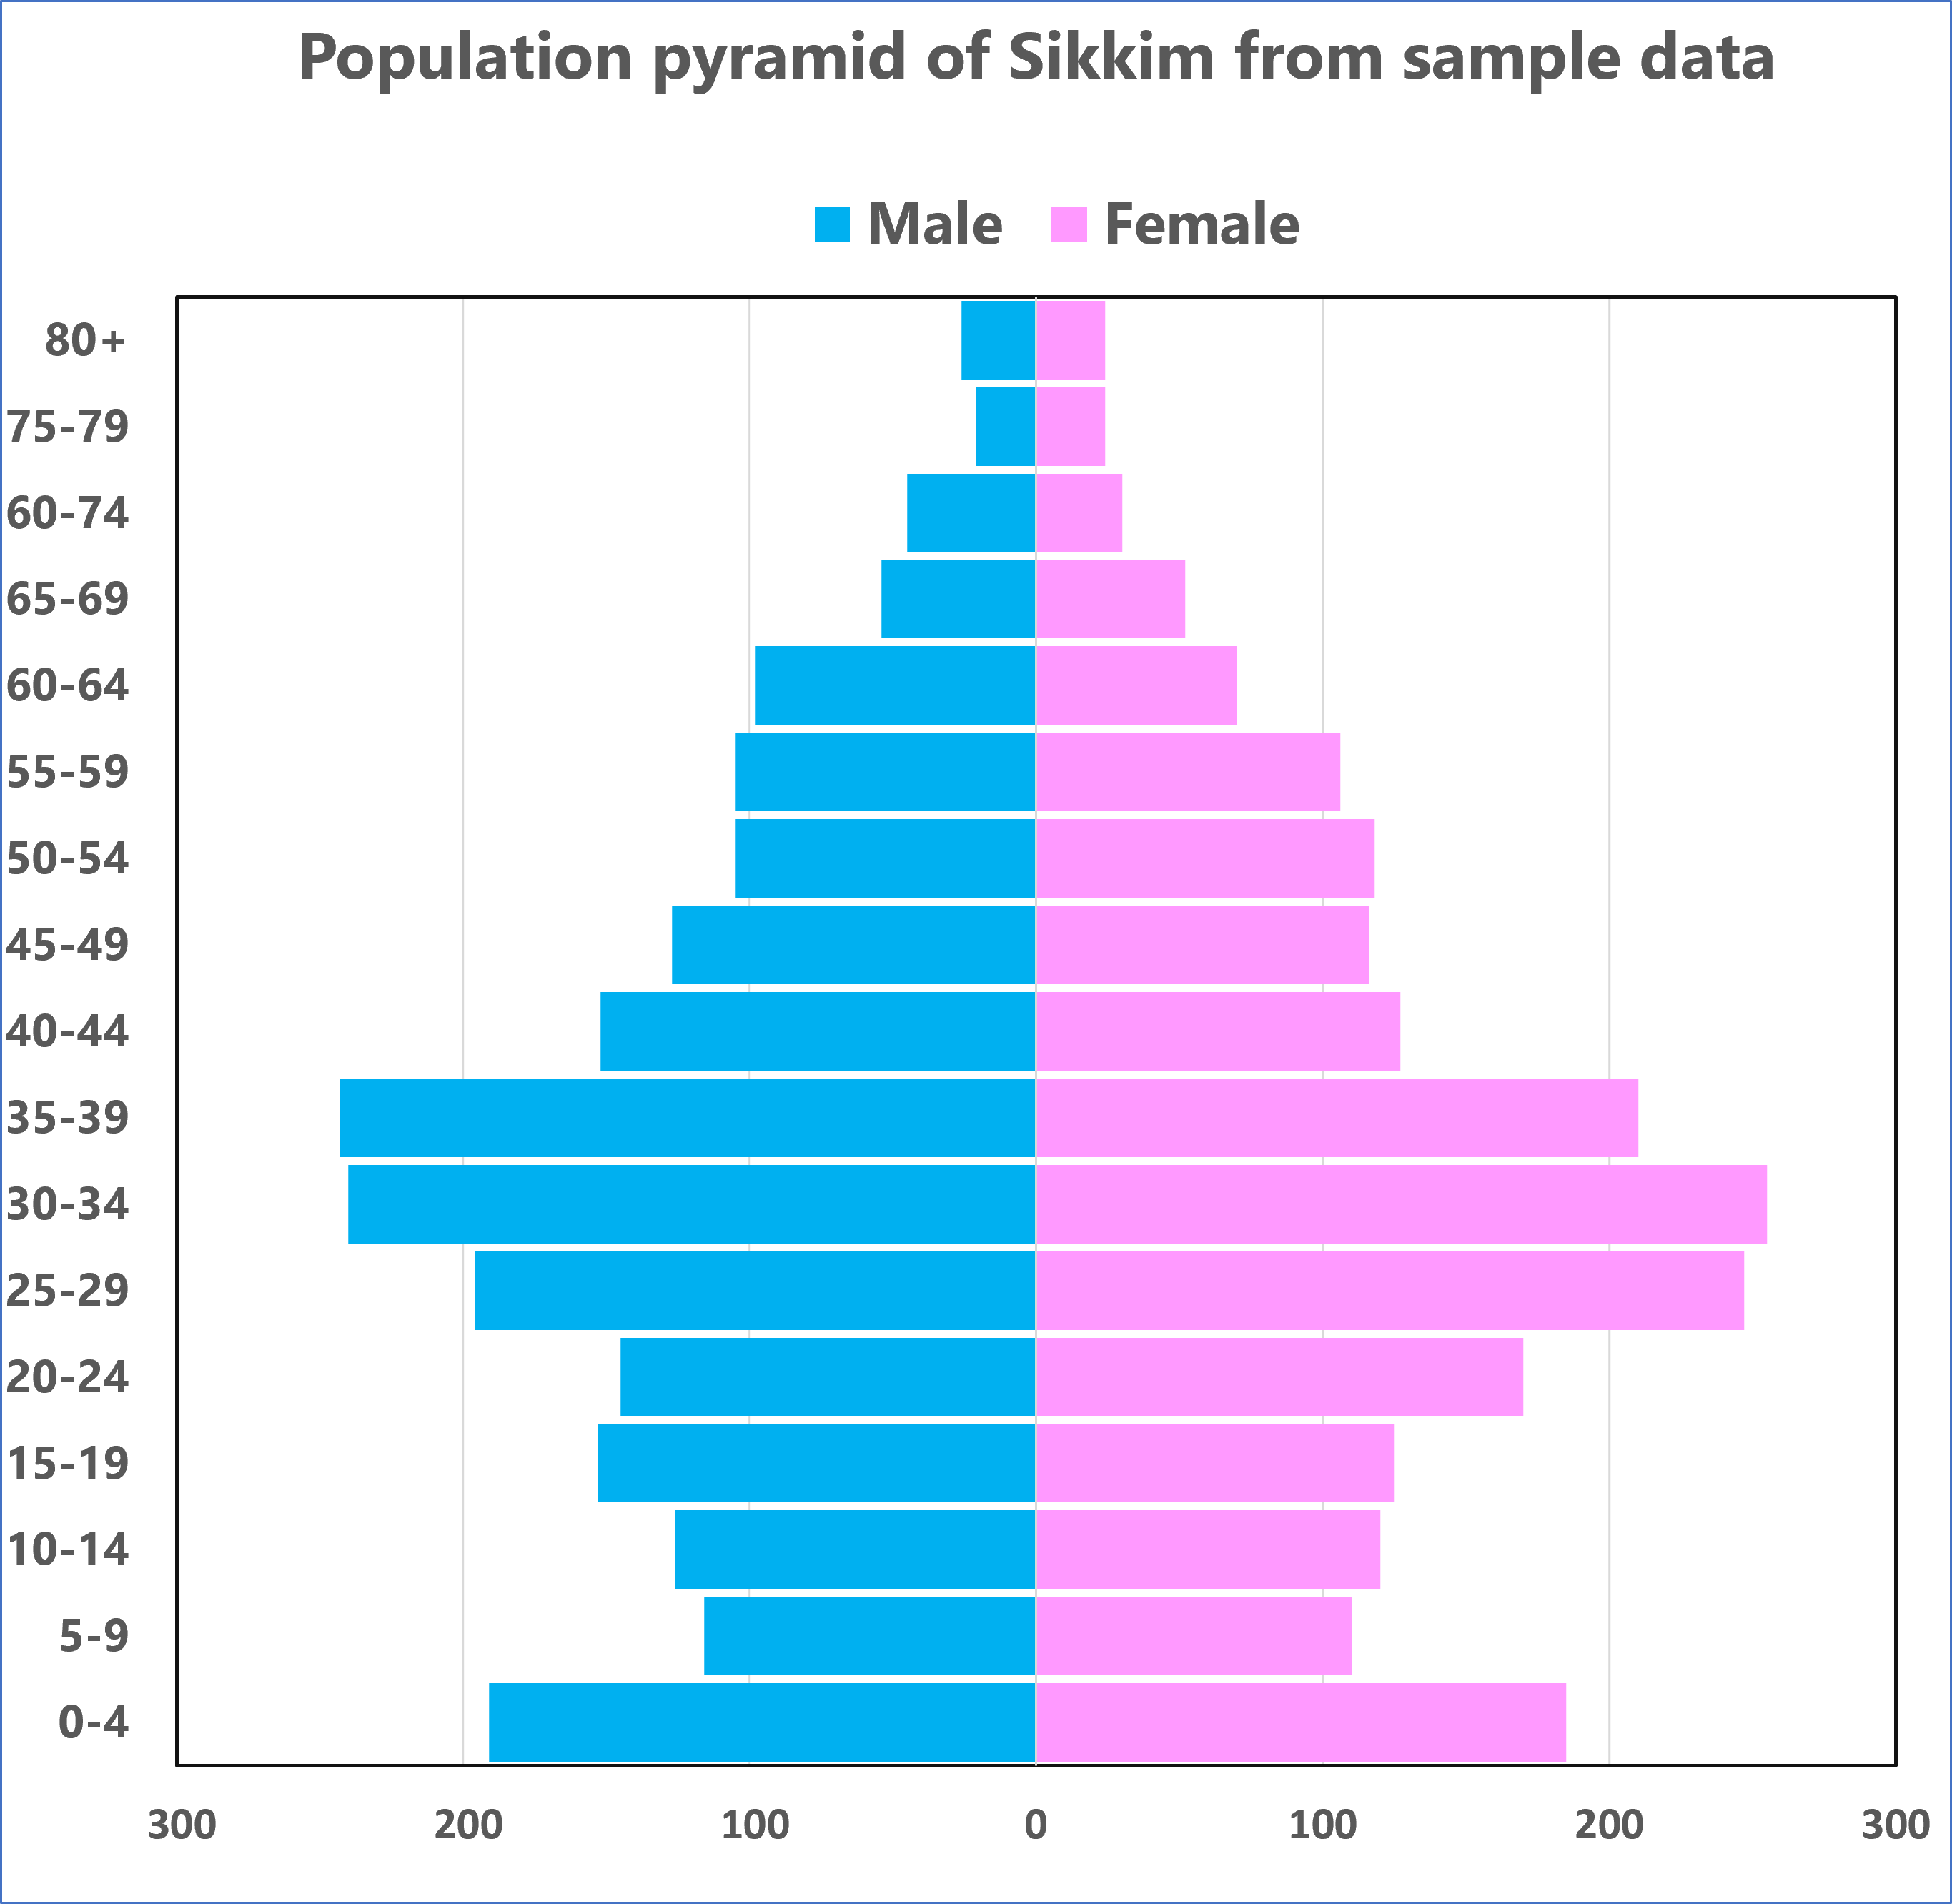
\includegraphics[width=0.45\linewidth]{sikpyramid.png}\caption{Age-sex structure of the two states (\% of the male and female population in each five-year age group)}
{\footnotesize\itshape Source: authors' calculations from NSS 80th Round (2025), Schedule 25.0, unit-level data.\par}
    \label{fig:placeholder}
    \end{figure}


\textbf{Age structure.} Rajasthan's pyramid is broad at the base: 25.3\% of persons are under 15 and 6.9\% are under 5. Sikkim's has a narrow base (under-5s are only 2.7\% of the population) and a bulge at ages 25--39. As a result Sikkim's median age is 5.0 years higher (95\% CI 3.5 to 6.5) and its total dependency ratio is 0.31 against 0.55: Sikkim has about 31 dependants per 100 working-age persons, Rajasthan about 55. Sikkim is therefore in a favourable position for the working-age share, but with so few children its age structure will keep ageing; Rajasthan has a larger share of children still to enter the labour force.


\textbf{Households and headship.} Households are larger in Rajasthan (4.53 members) than in Sikkim (3.38). The female-headed share is 13.1\% and 16.0\%; the intervals overlap, so we cannot call this a difference.


\textbf{Sex ratio, with a caution.} The estimated sex ratio is 973 [940, 1005] in Rajasthan and 871 [794, 947] in Sikkim. The Sikkim figure, and especially its urban value (700, interval 548 to 853), is sensitive to a few high-weight households and probably reflects male in-migration and sampling variability. The unweighted Sikkim sample is close to balanced (about 975). A household sample should not replace Census figures for this indicator.


\textbf{Composition.} Both states are about three-quarters rural. Rajasthan is 89\% Hindu and 9\% Muslim; Sikkim is 69\% Hindu, 22\% Buddhist and 7\% Christian. Scheduled Tribes are 34\% of Sikkim's persons against 14\% in Rajasthan, while Scheduled Castes are 19\% in Rajasthan against 7\% in Sikkim.


\section{Fertility, marriage and women's education}

We next look at the demographic processes behind these structures, namely fertility and marriage, and at women's schooling. Only the survey's pregnancy item and marital-status item are available, so fertility is a proxy (Section 2.3) and mortality cannot be examined.


\begin{table}[!htb]\centering
\caption{Fertility, marriage and education (estimate with 95\% CI)}
\rowcolors{2}{white}{zebra}
\begin{tabular}{>{\raggedright\arraybackslash}p{6.62cm}>{\raggedright\arraybackslash}p{4.77cm}>{\raggedright\arraybackslash}p{4.77cm}}
\toprule
\rowcolor{navy}\textcolor{white}{\textbf{Indicator}} & \textcolor{white}{\textbf{Rajasthan}} & \textcolor{white}{\textbf{Sikkim}} \\
\midrule
Pregnancy-based fertility index (TFI) & 2.10 [1.92, 2.29] & 0.80 [0.65, 0.96] \\
Mean age of reported pregnancy (years) & 26.6 [26.2, 27.0] & 30.7 [29.7, 31.7] \\
SMAM, women (years) & 22.9 [22.4, 23.3] & 27.4 [26.3, 28.6] \\
SMAM, men (years) & 26.6 [26.1, 27.2] & 31.4 [29.9, 32.9] \\
Gap in SMAM, men minus women (years) & 3.8 [3.2, 4.4] & 4.0 [2.3, 5.7] \\
Women aged 15--19 ever married (\%) & 6.2 [3.9, 8.5] & 0.3 [0.0, 0.7] \\
Women aged 20--24 ever married (\%) & 49.3 [44.3, 54.2] & 14.0 [4.2, 23.7] \\
Men aged 20--24 ever married (\%) & 21.4 [17.4, 25.4] & 8.0 [0.0, 17.1] \\
Not literate, women 25+ (\%) & 46.7 [44.2, 49.2] & 10.5 [7.0, 14.1] \\
Not literate, men 25+ (\%) & 19.3 [17.4, 21.2] & 6.4 [3.5, 9.2] \\
Secondary or higher, women 25+ (\%) & 24.0 [21.9, 26.0] & 55.0 [49.1, 60.9] \\
Secondary or higher, men 25+ (\%) & 46.6 [44.0, 49.1] & 59.6 [52.9, 66.4] \\
Parity index, secondary or higher (F/M) & 0.51 [0.48, 0.55] & 0.92 [0.82, 1.03] \\
Parity index, literacy ages 15+ (F/M) & 0.74 [0.72, 0.76] & 0.97 [0.93, 1.00] \\
\bottomrule
\end{tabular}
\begin{minipage}{\textwidth}\par\vspace{2pt}{\footnotesize\itshape Notes: secondary or higher includes secondary, higher secondary, diploma or certificate courses, graduate and postgraduate. Literate means any code other than ``not literate''.\par}\end{minipage}
\end{table}

\begin{figure}[!htb]\centering
\includegraphics[width=13.5cm]{figs/f2_fertility.png}
\caption{Age pattern of reported pregnancies among women aged 15--49 (shaded bands: 95\% CI)}
{\footnotesize\itshape Source: authors' calculations from NSS 80th Round (2025), Schedule 25.0, unit-level data.\par}
\end{figure}

\textbf{Fertility.} Rajasthan's index of 2.10 [1.92, 2.29] is close to the NFHS-5 total fertility rate of 2.0 for the state [2], which supports using the item as a proxy. Sikkim's index of 0.80 [0.65, 0.96] is lower than the latest value of 1.1 listed for Sikkim in the same table [2], so the proxy probably understates fertility there; the direction (very low fertility) is not in doubt, but the level is. The age profiles differ in shape as well as height: Rajasthan's peak is at ages 20--29, Sikkim's at 30--34, and the mean age of reported pregnancy is 26.6 versus 30.7 years.


\textbf{Fertility scenarios.} A simple benchmark helps interpret these levels. With a replacement-level total fertility of about 2.1 [9] and ignoring mortality and migration, each generation of women would be roughly the size of its mothers' generation. The table below shows what each level implies per generation. It is an illustration of arithmetic, not a projection.


\begin{table}[!htb]\centering
\caption{Illustrative generational replacement at different fertility levels}
\rowcolors{2}{white}{zebra}
\begin{tabular}{>{\raggedright\arraybackslash}p{6.92cm}>{\raggedright\arraybackslash}p{2.72cm}>{\raggedright\arraybackslash}p{6.52cm}}
\toprule
\rowcolor{navy}\textcolor{white}{\textbf{Scenario}} & \textcolor{white}{\textbf{Total fertility}} & \textcolor{white}{\textbf{Next generation relative to current (replacement = 1.00)}} \\
\midrule
\textbf{Rajasthan, survey proxy} & 2.10 & 1.00 \\
\textbf{Sikkim, survey proxy} & 0.80 & 0.38 \\
\textbf{Sikkim, NFHS-5 level (latest value listed [2])} & 1.10 & 0.52 \\
\bottomrule
\end{tabular}
\begin{minipage}{\textwidth}\par\vspace{2pt}{\footnotesize\itshape Notes: ratio = total fertility divided by 2.1, assuming a closed population and negligible mortality before the end of childbearing.\par}\end{minipage}
\end{table}

\textbf{Marriage.} Women in Rajasthan marry about 4.6 years earlier than in Sikkim (SMAM 22.9 against 27.4). 49\% of Rajasthani women aged 20--24 have ever married, compared with 14\% in Sikkim. In both states men marry about four years later than women (gap 3.8 and 4.0 years), so the difference between men's and women's marriage ages, a rough proxy for the spousal age gap, is similar even though the level of marriage age is very different.


\textbf{Education.} 47\% of Rajasthani women aged 25+ are not literate, against 19\% of men; in Sikkim the figures are 11\% and 6\%. Only 24\% of Rajasthani women aged 25+ have completed secondary schooling or more, half the male rate (parity index 0.51); in Sikkim the index is 0.92 and its interval includes parity. Because these are stocks of adults, they mostly record past schooling opportunities; they say little about current enrolment of girls.


\section{Gender differences in health indicators}

Here we ask whether illness, hospital use, vaccination and scheme coverage differ between women and men, after allowing for age. Ratios are female divided by male, so values below 1 mean a lower female rate.




\rowcolors{2}{white}{zebra}
\begin{longtable}{>{\raggedright\arraybackslash}p{6.62cm}>{\raggedright\arraybackslash}p{4.77cm}>{\raggedright\arraybackslash}p{4.77cm}}
\caption{Health indicators by sex (estimate with 95\% CI)}\\
\toprule
\rowcolor{navy}\textcolor{white}{\textbf{Indicator}} & \textcolor{white}{\textbf{Rajasthan}} & \textcolor{white}{\textbf{Sikkim}} \\
\midrule \endhead
\bottomrule \endlastfoot
Chronic ailment, age-std.: women (\%) & 7.0 [6.2, 7.8] & 6.2 [4.2, 8.3] \\
Chronic ailment, age-std.: men (\%) & 6.6 [5.9, 7.3] & 6.6 [4.3, 8.9] \\
\textbf{Chronic ailment, age-std.: ratio F/M} & 1.05 [0.90, 1.20] & 0.95 [0.56, 1.34] \\
Any other ailment in last 15 days, age-std.: women (\%) & 5.1 [4.3, 6.0] & 5.3 [2.6, 8.0] \\
Any other ailment in last 15 days, age-std.: men (\%) & 4.4 [3.7, 5.2] & 5.0 [2.8, 7.2] \\
\textbf{Any other ailment in last 15 days, age-std.: ratio F/M} & 1.17 [0.92, 1.41] & 1.05 [0.42, 1.67] \\
Hospitalised, age-std., all ages: women (\%) & 5.6 [5.3, 6.0] & 4.3 [3.4, 5.2] \\
Hospitalised, age-std., all ages: men (\%) & 2.4 [2.1, 2.7] & 2.3 [1.7, 2.8] \\
\textbf{Hospitalised, age-std., all ages: ratio F/M} & 2.34 [2.05, 2.63] & 1.91 [1.46, 2.36] \\
Hospitalised, age-std., excluding ages 15--49: women (\%) & 2.8 [2.3, 3.3] & 4.8 [2.9, 6.8] \\
Hospitalised, age-std., excluding ages 15--49: men (\%) & 3.5 [3.0, 4.1] & 3.2 [2.2, 4.2] \\
\textbf{Hospitalised, age-std., excluding ages 15--49: ratio F/M} & 0.79 [0.64, 0.95] & 1.51 [0.76, 2.26] \\
Hospitalised, ages 15--49: women (\%) & 7.5 [6.9, 8.1] & 4.1 [3.6, 4.7] \\
Hospitalised, ages 15--49: men (\%) & 1.6 [1.4, 1.9] & 1.7 [0.9, 2.4] \\
Any vaccine, ages 0--4: girls (\%) & 84.4 [80.4, 88.4] & 73.6 [46.6, 100] \\
Any vaccine, ages 0--4: boys (\%) & 83.4 [79.0, 87.8] & 88.1 [68.5, 100] \\
Covered by a health scheme: women (\%) & 77.7 [75.4, 80.1] & 17.8 [12.3, 23.4] \\
Covered by a health scheme: men (\%) & 76.7 [74.3, 79.1] & 19.3 [13.7, 25.0] \\
\end{longtable}
\par\vspace{2pt}{\footnotesize\itshape Notes: age-standardised to the average age distribution of the two states. Sikkim vaccine estimates rest on only 376 children aged 0--4, 185 of them girls.\par}

\begin{figure}[!htb]\centering
\includegraphics[width=15.8cm]{figs/f3_gender.png}
\caption{Female-to-male ratios for health, coverage and education indicators (parity = 1)}
{\footnotesize\itshape Source: authors' calculations from NSS 80th Round (2025), Schedule 25.0, unit-level data.\par}
\end{figure}

\textbf{Illness is not clearly gendered.} Chronic-ailment prevalence is similar for women and men in both states (female/male ratio 1.05 [0.90, 1.20] in Rajasthan and 0.95 [0.56, 1.34] in Sikkim). Women report more ailments in the last 15 days in Rajasthan (1.17), but the interval includes 1. Coverage by a health scheme is at parity in both states, and vaccination of children aged 0--4 shows no gap in Rajasthan.


\textbf{The headline hospitalisation gap is mostly childbirth.} Across all ages, women are hospitalised 2.3 times as often as men in Rajasthan and 1.9 times in Sikkim. At ages 15--49 the rate is 7.5\% for women and 1.6\% for men in Rajasthan. Removing ages 15--49 changes the picture in Rajasthan: the ratio falls to 0.79 [0.64, 0.95], i.e. women are \textit{less} likely than men to be hospitalised. The adjusted odds ratio for women (controlling for age, sector, expenditure quintile, social group and coverage) is 0.78 [0.65, 0.95]. In Sikkim the corresponding ratio is 1.51 [0.76, 2.26], which is imprecise and consistent with parity.


This is a pattern worth presenting carefully. Chronic and recent illness are not lower for women, so lower hospital use outside the childbearing years is \textit{consistent with} women receiving less inpatient care than their needs would warrant. The survey cannot prove that: hospital use depends on need that these items do not fully capture, on severity, and on who decides and pays. We therefore describe it as a gap to investigate, not as proof of discrimination.


\begin{table}[!htb]\centering
\caption{Selected adjusted odds ratios from weighted logistic regressions}
\rowcolors{2}{white}{zebra}
\begin{tabular}{>{\raggedright\arraybackslash}p{8.32cm}>{\raggedright\arraybackslash}p{3.92cm}>{\raggedright\arraybackslash}p{3.92cm}}
\toprule
\rowcolor{navy}\textcolor{white}{\textbf{Model (adjusted odds ratio, 95\% CI)}} & \textcolor{white}{\textbf{Rajasthan}} & \textcolor{white}{\textbf{Sikkim}} \\
\midrule
Chronic ailment: female vs male & 1.07 [0.89, 1.27] & 0.86 [0.52, 1.43] \\
Chronic ailment: richest vs poorest quintile & 1.87 [1.33, 2.64] & 1.21 [0.17, 8.49] \\
Hospitalised, excl. ages 15--49: female vs male & 0.78 [0.65, 0.95] & 1.52 [0.91, 2.53] \\
Hospitalised, excl. ages 15--49: richest vs poorest quintile & 1.76 [1.14, 2.72] & 1.39 [0.63, 3.07] \\
Hospitalised, excl. ages 15--49: covered vs not covered & 0.88 [0.64, 1.22] & 1.90 [1.14, 3.16] \\
Hospitalised, all ages: female vs male & 2.26 [1.99, 2.56] & 2.04 [1.60, 2.60] \\
\bottomrule
\end{tabular}
\begin{minipage}{\textwidth}\par\vspace{2pt}{\footnotesize\itshape Notes: all models control for age band, rural sector, expenditure quintile, social group and scheme coverage; standard errors clustered by FSU. Sample sizes: Rajasthan 39,802 (chronic) and 18,959 (hospitalisation excl. 15--49); Sikkim 4,232 and 1,726. Sikkim intervals are wide because of few events and 130 FSUs.\par}\end{minipage}
\end{table}

\section{Consumption patterns}

Consumption is measured by household usual consumer expenditure from Block 5 of the survey. We describe its level, the sources it comes from, and differences by sector and social group.


\begin{table}[!htb]\centering
\caption{Monthly per-capita consumer expenditure (MPCE), estimate with 95\% CI}
\rowcolors{2}{white}{zebra}
\begin{tabular}{>{\raggedright\arraybackslash}p{6.62cm}>{\raggedright\arraybackslash}p{4.77cm}>{\raggedright\arraybackslash}p{4.77cm}}
\toprule
\rowcolor{navy}\textcolor{white}{\textbf{Indicator (Rs per person per month)}} & \textcolor{white}{\textbf{Rajasthan}} & \textcolor{white}{\textbf{Sikkim}} \\
\midrule
10th percentile & 1,886 [1,791, 1,980] & 2,684 [2,140, 3,227] \\
Median & 3,032 [2,964, 3,101] & 4,583 [4,215, 4,952] \\
Mean & 3,492 [3,388, 3,596] & 5,272 [4,803, 5,742] \\
90th percentile & 5,556 [5,259, 5,852] & 9,125 [8,040, 10,210] \\
Median, rural & 2,857 [2,780, 2,933] & 4,333 [4,042, 4,624] \\
Median, urban & 3,745 [3,534, 3,956] & 6,042 [5,179, 6,904] \\
Median, Scheduled Tribe households & 2,510 [2,345, 2,675] & 5,000 [4,589, 5,411] \\
Median, Scheduled Caste households & 2,903 [2,773, 3,032] & 4,153 [3,115, 5,191] \\
Median, OBC households & 3,083 [2,992, 3,174] & 4,440 [4,097, 4,783] \\
Median, other households & 3,708 [3,478, 3,938] & 5,521 [3,538, 7,504] \\
Urban / rural ratio of medians & 1.31 [1.23, 1.40] & 1.39 [1.17, 1.62] \\
\bottomrule
\end{tabular}
\begin{minipage}{\textwidth}\par\vspace{2pt}{\footnotesize\itshape Notes: MPCE = household usual consumer expenditure / household size, person-weighted. Not comparable with household consumption expenditure survey figures.\par}\end{minipage}
\end{table}

\begin{table}[!htb]\centering
\caption{Composition of household usual consumer expenditure (household-weighted)}
\rowcolors{2}{white}{zebra}
\begin{tabular}{>{\raggedright\arraybackslash}p{6.62cm}>{\raggedright\arraybackslash}p{4.77cm}>{\raggedright\arraybackslash}p{4.77cm}}
\toprule
\rowcolor{navy}\textcolor{white}{\textbf{Share of household expenditure (\%)}} & \textcolor{white}{\textbf{Rajasthan}} & \textcolor{white}{\textbf{Sikkim}} \\
\midrule
Purchased goods and services (monthly) & 72.6 [71.6, 73.5] & 79.0 [76.5, 81.4] \\
Home-grown stock (imputed) & 12.0 [11.2, 12.8] & 5.1 [3.3, 6.9] \\
Wages in kind, gifts, free collection (imputed) & 3.3 [3.1, 3.6] & 1.2 [0.8, 1.6] \\
Clothing, footwear and durables (annual, per month) & 12.1 [11.5, 12.7] & 14.8 [12.9, 16.6] \\
\hspace{1.2em}of which clothing and footwear & 6.7 [6.5, 7.0] & 9.6 [8.3, 10.8] \\
\hspace{1.2em}of which durables & 5.4 [4.8, 5.9] & 5.2 [3.7, 6.7] \\
Home-grown share, rural households & 17.1 [16.2, 18.0] & 7.4 [4.8, 10.0] \\
Home-grown share, urban households & 2.7 [1.8, 3.6] & 0.4 [0.0, 0.8] \\
Households paying a medical insurance premium (\%) & 6.3 [5.1, 7.6] & 12.7 [7.5, 17.9] \\
\bottomrule
\end{tabular}
\begin{minipage}{\textwidth}\par\vspace{2pt}{\footnotesize\itshape Notes: shares of total household usual consumer expenditure. The survey does not split expenditure into food and non-food, so Engel-type analysis is not possible with these files.\par}\end{minipage}
\end{table}

\textbf{Levels.} The median Sikkimese resident spends about 1.5 times as much per month as the median Rajasthani (Rs 4,583 against Rs 3,032), and the cut-off for Sikkim's poorest tenth (Rs 2,684) is above the cut-off for Rajasthan's poorest fifth (Rs 2,257). Prices differ between the states, so these are nominal comparisons. Urban medians exceed rural by 31\% in Rajasthan and 39\% in Sikkim.


\textbf{Social groups.} In Rajasthan, Scheduled Tribe households have a median MPCE of Rs 2,510, about 32\% below other households (Rs 3,708). In Sikkim there is no clear ranking: the median for Scheduled Tribe households (Rs 5,000) is not below the ``other'' group, whose estimate is imprecise (3,538 to 7,504).


\textbf{Composition.} Home-grown consumption makes up 12\% of Rajasthani household expenditure (17\% in rural households) against 5\% in Sikkim, consistent with a larger role for own production in rural Rajasthan. Sikkim households put a larger share into clothing, footwear and durables (15\% against 12\%), and twice as many Sikkim households report paying an insurance premium (13\% against 6\%), despite Sikkim's far lower coverage by public schemes (Section 8): privately bought and employer-linked cover matter relatively more there.


\section{Inequality in consumption and health}

We measure inequality in two ways: the dispersion of consumption (Gini coefficient, Lorenz curve, percentile ratios) and the distribution of health outcomes and coverage along the expenditure ranking (concentration indices).


\begin{table}[!htb]\centering
\caption{Inequality in MPCE (estimate with 95\% CI)}
\rowcolors{2}{white}{zebra}
\begin{tabular}{>{\raggedright\arraybackslash}p{6.62cm}>{\raggedright\arraybackslash}p{4.77cm}>{\raggedright\arraybackslash}p{4.77cm}}
\toprule
\rowcolor{navy}\textcolor{white}{\textbf{Inequality measure}} & \textcolor{white}{\textbf{Rajasthan}} & \textcolor{white}{\textbf{Sikkim}} \\
\midrule
Gini coefficient, all & 0.255 [0.242, 0.268] & 0.258 [0.222, 0.293] \\
Gini, rural & 0.209 [0.195, 0.223] & 0.248 [0.197, 0.298] \\
Gini, urban & 0.298 [0.278, 0.318] & 0.217 [0.185, 0.249] \\
90th / 10th percentile ratio & 2.95 [2.75, 3.15] & 3.40 [2.64, 4.16] \\
80th / 20th percentile ratio & 1.88 [1.81, 1.95] & 2.01 [1.71, 2.30] \\
Share of consumption: top 10\% of persons (\%) & 22.4 [21.4, 23.5] & 21.2 [18.4, 24.0] \\
Share of consumption: bottom 40\% of persons (\%) & 24.9 [24.1, 25.6] & 24.4 [22.0, 26.8] \\
Share of consumption by quintile Q1 to Q5 (\%) & 10.3 / 14.5 / 17.4 / 21.5 / 36.3 & 9.6 / 14.9 / 17.6 / 22.1 / 35.9 \\
\bottomrule
\end{tabular}
\end{table}

\begin{figure}[!htb]\centering
\includegraphics[width=16.2cm]{figs/f4_inequality.png}
\caption{Lorenz curves of MPCE and the level of MPCE in each state}
{\footnotesize\itshape Source: authors' calculations from NSS 80th Round (2025), Schedule 25.0, unit-level data.\par}
\end{figure}

\textbf{Consumption inequality is about the same.} The Gini coefficients are 0.255 and 0.258; the difference (Sikkim minus Rajasthan, 0.003) has a 95\% interval of $-$0.035 to 0.041, so there is no evidence that the states differ. The Lorenz curves are nearly indistinguishable even though the levels differ by 50\%. The top 10\% of persons account for 22\% of consumption in Rajasthan and 21\% in Sikkim. Beneath the similar totals the geography differs: Rajasthan's urban Gini (0.298) is well above its rural (0.209), whereas in Sikkim the rural Gini (0.248) exceeds the urban (0.217). Absolute differences in expenditure are what matter for welfare, so a similar Gini on a lower level of consumption leaves Rajasthan's poorest households with much less in rupee terms. The Gini levels are specific to this expenditure concept and should not be compared with values from other surveys.


\begin{figure}[!htb]\centering
\includegraphics[width=16.6cm]{figs/f5_quintile.png}
\caption{Health outcomes and coverage by MPCE quintile (age-standardised where marked; vertical bars: 95\% CI)}
{\footnotesize\itshape Source: authors' calculations from NSS 80th Round (2025), Schedule 25.0, unit-level data.\par}
\end{figure}

\begin{figure}[!htb]\centering
\includegraphics[width=15.8cm]{figs/f7_concentration.png}
\caption{Concentration indices of coverage and health outcomes (rank by MPCE)}
{\footnotesize\itshape Source: authors' calculations from NSS 80th Round (2025), Schedule 25.0, unit-level data.\par}
\end{figure}

\textbf{Health inequality.} Chronic ailment is reported more often by richer Rajasthanis: the prevalence rises from 5.1\% in Q1 to 9.3\% in Q5 and the standardised concentration index is 0.119 [0.076, 0.162]. A gradient of this kind in self-reported morbidity commonly reflects better diagnosis and awareness among richer groups rather than better health, so it should not be read as the rich being sicker. In Sikkim the index is 0.023 [$-$0.164, 0.211], i.e. uninformative.


Hospitalisation has no clear income gradient in either state (concentration index $-$0.018 [$-$0.057, 0.022] in Rajasthan, $-$0.006 [$-$0.104, 0.092] in Sikkim). Excluding childbirth ages, however, richer Rajasthanis are more likely to be hospitalised (richest vs poorest quintile adjusted odds ratio 1.76 [1.14, 2.72]), a possible sign of unmet need among poorer households that is hidden in the all-age rate.


\section{Health-financing coverage: a policy comparison}

The last comparison concerns how health care is financed in each state. We describe who is covered and by which type of scheme, and how coverage relates to hospital use.


\begin{figure}[!htb]\centering
\includegraphics[width=14.5cm]{figs/f6_schemes.png}
\caption{Coverage by type of health financing scheme (\% of persons)}
{\footnotesize\itshape Source: authors' calculations from NSS 80th Round (2025), Schedule 25.0, unit-level data.\par}
\end{figure}

\begin{table}[!htb]\centering
\caption{Coverage by any health financing scheme, by group (estimate with 95\% CI)}
\rowcolors{2}{white}{zebra}
\begin{tabular}{>{\raggedright\arraybackslash}p{6.62cm}>{\raggedright\arraybackslash}p{4.77cm}>{\raggedright\arraybackslash}p{4.77cm}}
\toprule
\rowcolor{navy}\textcolor{white}{\textbf{Any health scheme (\%)}} & \textcolor{white}{\textbf{Rajasthan}} & \textcolor{white}{\textbf{Sikkim}} \\
\midrule
All persons & 77.2 [75.0, 79.4] & 18.6 [13.4, 23.8] \\
Rural & 79.1 [76.4, 81.9] & 17.4 [11.3, 23.5] \\
Urban & 72.1 [68.3, 75.9] & 22.2 [10.8, 33.6] \\
Women & 77.7 [75.4, 80.1] & 17.8 [12.3, 23.4] \\
Men & 76.7 [74.3, 79.1] & 19.3 [13.7, 25.0] \\
Scheduled Tribe & 78.2 [71.5, 84.9] & 19.2 [12.1, 26.3] \\
Scheduled Caste & 77.9 [73.5, 82.4] & 9.6 [0.0, 20.4] \\
OBC & 78.1 [75.1, 81.1] & 16.4 [9.6, 23.2] \\
Others & 73.2 [68.5, 77.8] & 36.8 [16.4, 57.3] \\
Poorest quintile (Q1) & 76.3 [71.1, 81.6] & 13.7 [2.2, 25.3] \\
Richest quintile (Q5) & 76.4 [72.0, 80.8] & 29.4 [16.1, 42.8] \\
\bottomrule
\end{tabular}
\begin{minipage}{\textwidth}\par\vspace{2pt}{\footnotesize\itshape Notes: one scheme code is recorded per person; people with several covers appear under one. Sikkim subgroup estimates are imprecise.\par}\end{minipage}
\end{table}

\textbf{Level and design.} 77\% of Rajasthan's population is covered by some scheme and 19\% of Sikkim's (difference 59 percentage points, interval 53 to 64). In Rajasthan the State Health Insurance Scheme alone covers 53\% and AB-PMJAY 19\%. In Sikkim the largest single category is employer or government-employee schemes (9\%), with AB-PMJAY at 4\% and a state scheme at 2\%; 81\% of persons are not covered by any scheme.


\textbf{Equity of coverage.} Rajasthan's broad design shows up as flat coverage: it is 76\% in the poorest quintile and 76\% in the richest, with a concentration index of 0.003 [$-$0.013, 0.019]. Within it, AB-PMJAY is pro-poor (index $-$0.116 [$-$0.177, $-$0.055]), while employer and government-employee cover is strongly pro-rich (index 0.55 [0.45, 0.65]). In Sikkim, coverage climbs from 14\% in Q1 to 29\% in Q5 (index 0.16 [$-$0.01, 0.33], whose interval just includes zero). Coverage is similar for women and men in both states, and in Rajasthan it varies little across social groups (73\% to 78\%) but is higher in rural than urban areas (79\% against 72\%).


\textbf{Is coverage related to hospital use?} The age-sex-standardised hospitalisation rate of covered persons relative to uncovered persons is 0.95 [0.78, 1.11] in Rajasthan and 1.53 [0.91, 2.14] in Sikkim. After adjustment (excluding childbirth ages) the odds ratio for coverage is 0.88 [0.64, 1.22] in Rajasthan and 1.90 [1.14, 3.16] in Sikkim. In Rajasthan we find no measurable difference. In Sikkim the covered are more likely to have been hospitalised, which is more plausibly selection (people with health needs, or salaried employees with reimbursement rights, are more likely to hold cover) than an effect of the schemes.


\textbf{What this does and does not show.} The data support a clear descriptive conclusion: Rajasthan has built broad, income-neutral coverage, whereas Sikkim's coverage is low and skewed toward richer and salaried households. They do not show that coverage improves health, or even that it protects households financially. For that we would need spending and reimbursement records from the hospitalisation-episode file. Low insurance coverage in Sikkim also does not mean low protection, since care in public facilities can be free or subsidised without involving an insurance scheme; the survey does not capture that. A proper policy evaluation would compare the same states before and after the scheme, for example against the previous NSS health round, which a single 2025 cross-section cannot do.


\section{Limitations and what further data would allow}

\begin{itemize}
\item \textbf{No mortality data in the files supplied.} Life tables and life expectancy need deaths by age (the survey's Level 3 file, Block 4, records the sex and age at death of deceased household members). With that file, age-specific death rates could be formed against the Block 3 population and an abridged life table built for each state.
\item \textbf{No expenditure on treatment.} Out-of-pocket spending, reimbursement and catastrophic expenditure sit in the hospitalisation-episode level (Blocks 6 and 7), which was not supplied. Financial protection, the central question for the scheme comparison, remains open.
\item \textbf{Proxy for fertility.} The pregnancy item has no stated reference period in the layout; our reading is supported by the Rajasthan match to NFHS-5 but not by Sikkim, so fertility levels should be treated as indicative.
\item \textbf{Small Sikkim sample.} With 130 FSUs and 1,033 households, Sikkim estimates for subgroups (sex ratios by sector, vaccination of girls, concentration indices) have wide intervals. Absence of a significant difference is not evidence of no difference.
\item \textbf{Self-reported morbidity and cross-section data.} Ailments and hospitalisation are self-reported, recall-dependent and influenced by awareness; associations are not causal.
\item \textbf{Consumption concept.} MPCE here comes from a health survey, lacks a food/non-food split, and is in nominal terms without a price adjustment between states.
\item \textbf{One coverage code per person.} Overlapping covers cannot be separated.
\end{itemize}

\section{Conclusions}

Rajasthan and Sikkim illustrate two points on the demographic and health-financing spectrum. Rajasthan is young, rural, higher-fertility and has large gender gaps in marriage age and schooling, but has extended health-scheme coverage widely and evenly across income groups. Sikkim is older, has very low fertility, narrower gender gaps in education and higher consumption, but its health-scheme coverage is low and favours richer, salaried households. Consumption inequality is similar in the two states. Within health, the most policy-relevant finding is that women in Rajasthan are less likely than men to be hospitalised outside the childbearing ages despite similar illness reports, a pattern that merits follow-up with the expenditure and episode data.


\begin{table}[!htb]\centering
\caption{Scorecard of differences (Sikkim minus Rajasthan)}
\rowcolors{2}{white}{zebra}
\begin{tabular}{>{\raggedright\arraybackslash}p{2.32cm}>{\raggedright\arraybackslash}p{5.92cm}>{\raggedright\arraybackslash}p{7.92cm}}
\toprule
\rowcolor{navy}\textcolor{white}{\textbf{Dimension}} & \textcolor{white}{\textbf{Indicator}} & \textcolor{white}{\textbf{Sikkim vs Rajasthan}} \\
\midrule
Demography & Median age (years) & Higher in Sikkim (+5.0; 95\% CI +3.5 to +6.5) \\
Demography & Total dependency ratio & Lower in Sikkim ($-$0.24; 95\% CI $-$0.30 to $-$0.18) \\
Fertility & Fertility index (TFI) & Lower in Sikkim ($-$1.30; 95\% CI $-$1.54 to $-$1.06) \\
Gender & Women's age at marriage (SMAM, years) & Higher in Sikkim (+4.6; 95\% CI +3.3 to +5.8) \\
Gender & Female/male secondary-plus parity & Higher in Sikkim (+0.41; 95\% CI +0.30 to +0.52) \\
Health & Chronic ailment, age-std. (pp) & No clear difference ($-$0.3 pp; 95\% CI $-$2.3 to +1.7) \\
Health & Hospitalisation, age-std. (pp) & Lower in Sikkim ($-$0.8 pp; 95\% CI $-$1.4 to $-$0.1) \\
Policy & Any health scheme (pp) & Lower in Sikkim ($-$58.6 pp; 95\% CI $-$64.2 to $-$52.9) \\
Consumption & Median MPCE (Rs) & Higher in Sikkim (+1551; 95\% CI +1177 to +1925) \\
Inequality & Gini coefficient & No clear difference (+0.003; 95\% CI $-$0.035 to +0.041) \\
\bottomrule
\end{tabular}
\begin{minipage}{\textwidth}\par\vspace{2pt}{\footnotesize\itshape Notes: ``clear'' means the 95\% interval for the difference excludes zero (states treated as independent samples); pp = percentage points.\par}\end{minipage}
\end{table}

\newpage
\nocite{*}
\bibliographystyle{unsrt}
\bibliography{ref}

\section*{R code}
The codes for the simulations can be found in this repository \cite{github-repo}.
\clearpage


\section*{Appendix A. Variables used and their codes}\addcontentsline{toc}{section}{Appendix A. Variables used and their codes}

\begin{center}
\rowcolors{2}{white}{zebra}
\begin{tabular}{>{\raggedright\arraybackslash}p{2.92cm}>{\raggedright\arraybackslash}p{5.92cm}>{\raggedright\arraybackslash}p{7.32cm}}
\toprule
\rowcolor{navy}\textcolor{white}{\textbf{Variable}} & \textcolor{white}{\textbf{Meaning (from the data layout)}} & \textcolor{white}{\textbf{Coding used in this report}} \\
\midrule
\textbf{sec} & Sector & 1 = rural, 2 = urban (rural-only household types appear only under 1) \\
\textbf{hhsz, umce} & Household size; household usual consumer expenditure (Rs per month) & MPCE = umce / hhsz; umce = b5i7 + b5i8 + b5i9 + (b5i10 + b5i11)/12 (checked to within Rs 0.5) \\
\textbf{b5i2, b5i3} & Religion; social group & Religion 1 Hindu, 2 Islam, 3 Christian, 4 Sikh, 5 Jain, 6 Buddhist; social group 1 ST, 2 SC, 3 OBC, 9 others \\
\textbf{b5i6, b5i5} & Medical insurance premium (Rs); outbreak of communicable disease in the community & Premium greater than 0 = pays a premium; 1 = outbreak reported \\
\textbf{b3c3, b3c4, b3c5} & Relation to head; sex; age (years) & Relation 1 = head; sex 1 male, 2 female, 3 transgender \\
\textbf{b3c6} & Marital status & 1 = never married; used for SMAM and ever-married shares \\
\textbf{b3c7} & Highest education level & 01 = not literate; secondary or higher = 06, 07, 08, 10, 11, 12, 13 \\
\textbf{b3c8} & Whether received any vaccine & 1 = yes, 2 = no (children 0--4) \\
\textbf{b3c9} & Whether hospitalised & 1 = yes. Reference period not stated in the layout \\
\textbf{b3c11} & Whether pregnant (women 15--49) & 1 = yes. Basis for the fertility index \\
\textbf{b3c13} & Communicable disease suffered & 19 = none \\
\textbf{b3c14, b3c15} & Chronic ailment; other ailment in the last 15 days & 1 = yes, 2 = no \\
\textbf{b3c17} & Covered by a health financing scheme & 1 AB-PMJAY, 2 State Health Insurance Scheme, 3 ESIS/ESIC, 4 CGHS/ECHS and other central schemes, 5 state-supported employee reimbursement, 6 PSU employer, 7 other employer, 10 private insurance only, 19 not covered. ``Employer / govt. employee'' in the report = codes 3 to 7 \\
\textbf{final\_weight, fsu, strat\_var} & Survey weight (multiplier / 100); first-stage unit; stratum & Used for all estimates; FSU and stratum define the bootstrap design \\
\bottomrule
\end{tabular}
\end{center}

\vspace{6pt}

\section*{Appendix B. Hospitalisation, weighted and unweighted}\addcontentsline{toc}{section}{Appendix B. Hospitalisation, weighted and unweighted}

\begin{center}
\rowcolors{2}{white}{zebra}
\begin{tabular}{>{\raggedright\arraybackslash}p{7.32cm}>{\raggedright\arraybackslash}p{4.42cm}>{\raggedright\arraybackslash}p{4.42cm}}
\toprule
\rowcolor{navy}\textcolor{white}{\textbf{}} & \textcolor{white}{\textbf{Rajasthan}} & \textcolor{white}{\textbf{Sikkim}} \\
\midrule
\textbf{Persons recorded as hospitalised (unweighted)} & 5,852 (14.7\%) & 800 (18.9\%) \\
\textbf{Weighted share hospitalised, all ages (\%)} & 3.9 [3.6, 4.1] & 3.1 [2.6, 3.7] \\
\textbf{Households by second-stage stratum 1 / 2 / 3} & 1866 / 3610 / 2166 & 231 / 532 / 270 \\
\bottomrule
\end{tabular}
\end{center}

{\footnotesize\itshape The gap between unweighted and weighted shares shows why unweighted tabulations of these files would be badly biased.\par}
\end{document}
